\documentclass{diploma}

\student{Харьков Павел Александрович}
\group{М8О-406Б-19}
\theme{Программа заполнения медицинской карты отделения неотложной медицинской помощи}

\supervisor{Пивоваров Дмитрий Евгеньевич}
\firstConsultant{}
\secondConsultant{}
\reviewer{}

\faculty{№ 8 <<Компьютерные науки и прикладная математика>>}
\department{806}
\speciality{01.03.02 <<Прикладная математика и информатика>>}
\profile{Информатика}

\departmentFullName{№ 806}
\headOfDepartment{Крылов Сергей Сергеевич}

% Дата. Оставляем пустое место для дня
\date{\uline{\hspace{24pt}} мая \the\year\ года}

\newacronym{api}{API}{Application Programming Interface}
\newacronym{http}{HTTP}{Hypertext Transfer Protocol}
\newacronym{maui}{MAUI}{Multi-platform App UI}
\newacronym{mvvm}{MVVM}{Model-View-ViewModel}
\newacronym{rest}{REST}{Representational State Transfer}
\newglossaryentry{id1}{ % Нужны разные id, можно ставить просто последовательно
    name={Backend},
    description={логика работы сайта, скрытая от пользователя} 
}
\newglossaryentry{id2}{
    name={МКБ},
    description={Международная классификация болезней} 
}
\newglossaryentry{id3}{
    name={$S^{2}$},
    description={формула в списке обозначений} 
}


\addbibresource{main.bib}

% Иллюстрации всегда по центру
\makeatletter
\g@addto@macro\@floatboxreset\centering
\makeatother

\begin{document}
    \maketitle

    % \includepdf[pages=-]{extra/task} % Задание
    \setcounter{page}{2} % Устанавливает счётчик страниц

    \abstract % Структурный элемент: РЕФЕРАТ

 % Реферат

    \tableofcontents % Содержание 
    \termsanddefenitions % Термины и определения
    \listofabbreviations % Перечень сокращений и обозначений
 
    \introduction % Структурный элемент: ВВЕДЕНИЕ

В современном мире медицинская отрасль активно развивается, и с каждым годом повышается необходимость во внедрении информационных технологий для упрощения и ускорения рабочих процессов. Одним из важнейших аспектов работы медицинских учреждений является отделение неотложной медицинской помощи, где обеспечение оперативного доступа к информации о пациентах, их медицинских картах, а также возможность быстро создавать и редактировать карты являются критически важными. 

С учетом этого, разработка программы заполнения медицинской карты отделения неотложной медицинской помощи представляет собой актуальную и значимую задачу. Создание мобильного приложения, которое будет обеспечивать доступ к медицинским картам и справочникам в удобном и быстром формате, способствует повышению качества предоставления медицинской помощи и снижению вероятности ошибок врачей при заполнении карт. Кроме того, реализация функционала автоматической синхронизации данных с сервером и возможность автономной работы с использованием локальной базы данных SQLite увеличивают надежность и доступность системы в условиях, когда стабильное подключение к интернету может быть ограничено.

Целью данной выпускной квалификационной работы является разработка и реализация мобильного приложения для заполнения медицинской карты отделения неотложной медицинской помощи.

Для достижения данной цели были сформулированы следующие задачи:
\begin{itemize}
    \item Изучение и сравнение существующих фреймворков для разработки мобильных приложений.

    \item Анализ требований к приложению и проектирование его архитектуры, включая определение основных сущностей, связей между ними и функциональных возможностей программы.

    \item Создание интерактивного макета интерфейса приложения в Figma.

    \item Разработка базы данных для приложения.
    
    \item Разработка программы, включая реализацию авторизации и регистрации пользователей, функций поиска карт и справочников, создания и редактирования медицинских карт, а также интеграцию с сервером через API для синхронизации данных.

    \item Тестирование разработанного приложения с использованием xUnit, включая проверку функций регистрации, авторизации, поиска, работы с медицинскими картами и генерации вопросов.

    \item Анализ возможностей дальнейшего развития и улучшения программы, определение перспективных направлений работы и их значимости для медицинской отрасли.
\end{itemize}
 % Введение

    % Название разделов -- все прописные
\section{ТЕОРЕТИЧЕСКОЕ ОБОСНОВАНИЕ РАЗРАБОТКИ БАЗЫ ДАННЫХ}

\subsection{Анализ предметной области}

Анализ предметной области является первым этапом в проектировании базы данных, в ходе которого выделяются основные объекты и их свойства, определяются первоначальные требования и границы проекта, чтобы разработать эффективную и безопасную базу данных.

Предметной областью разрабатываемой модели данных является система заполнения электронных медицинских карт для отделения неотложной медицинской помощи.

Скорая медицинская помощь (СМП) – вид медицинской помощи, оказываемой гражданам при заболеваниях, несчастных случаях, травмах, отравлениях и других состояниях, требующих срочного медицинского вмешательства.

Отделение неотложной (экстренной) медицинской помощи больницы является структурным подразделением многопрофильной больницы, которое в круглосуточном режиме оказывает экстренную (неотложную) медицинскую помощь.

Медицинская помощь включает в себя процедуру проведения осмотра, непосредственно манипуляции по оказанию медицинской помощи, а также консультирование пациента по с целью определения наиболее эффективного, безопасного и экономически оправданного курса лечения.

ОНМП осуществляет следующие функции:

\begin{itemize}
    \item прием пациентов с острыми заболеваниями, несчастными случаями, травмами, отравлениями и другими состояниями, требующими немедленной медицинской помощи;
    \item проведение первичной медицинской диагностики и оценки состояния пациента, осуществление мер, направленных на стабилизацию состояния пациента;
    \item предоставление неотложной медицинской помощи, включая проведение лечебных манипуляций, инъекций, переливание крови, а также оказание психологической помощи;
    \item организация и координация работы других специалистов и служб в медицинском учреждении, если необходимо;
    \item подготовка пациента к транспортировке в стационар для дальнейшего лечения;
    \item соблюдение всех медицинских стандартов и требований, направленных на обеспечение безопасности пациентов и медицинского персонала;
    \item организация транспортировки пациентов в случае необходимости;
    \item обеспечение работы необходимого медицинского оборудования, инструментов, материалов и медикаментов, необходимых для оказания неотложной медицинской помощи,
    \item проведение медицинской документации, включая учет медицинских случаев, регистрацию историй болезни и медицинских записей;
    \item обеспечение мониторинга и контроля за состоянием пациентов, находящихся на лечении в отделении неотложной (экстренной) медицинской помощи;
    \item обучение медицинского персонала и сотрудников отделения неотложной медицинской помощи новым методам лечения и диагностики;
    \item сотрудничество и консультации с другими медицинскими учреждениями, специалистами и службами для повышения качества оказываемой медицинской помощи.
\end{itemize}

Отделение неотложной (экстренной) медицинской помощи является ключевым звеном в системе оказания медицинской помощи населению и обеспечивает быстрое и эффективное лечение при острых заболеваниях и травмах.

Базы данных для неотложной медицинской помощи являются критически важным элементом в работе современных медицинских учреждений. Они позволяют эффективно организовывать, хранить и обрабатывать медицинскую информацию, ускоряя процессы принятия решений и повышая качество медицинской помощи.

Основным требованием к базе данных для неотложной медицинской помощи является ее способность оперативно и точно хранить медицинскую информацию о пациентах. Эта информация может включать данные о медицинской истории пациента, диагнозе, принятых мероприятиях, результатах обследований и лекарственном лечении.

Для эффективного управления медицинской информацией в базе данных неотложной медицинской помощи необходима специализированная система управления базами данных (СУБД). Существует множество СУБД, которые могут использоваться для этой цели, включая Oracle, MySQL, Microsoft SQL Server, PostgreSQL и др.

Также необходимо учитывать специфику работы медицинских учреждений, которые могут иметь различные требования к хранению и обработке медицинской информации. Например, больницы могут иметь разные отделения, каждое из которых может иметь свои особенности в обработке информации. Кроме того, необходимо учитывать возможность интеграции с другими системами, такими как системы управления ресурсами и планирования процессов.

Важно также отметить, что база данных для неотложной медицинской помощи должна соответствовать требованиям законодательства в области защиты персональных данных, таких как Федеральный закон от 27 июля 2006 года № 152-ФЗ «О персональных данных». Регулярное обновление и адаптация базы данных к изменениям в законодательстве помогут поддерживать соответствие нормам и предотвращать правовые проблемы.

Исследования показывают, что эффективное использование баз данных в медицинских учреждениях может значительно улучшить качество медицинской помощи и снизить затраты на ее оказание. Например, использование баз данных может уменьшить количество ошибок в принятии решений, сократить время, необходимое для оказания медицинской помощи, и повысить точность диагностики.

На текущий момент существует множество различных подходов к проектированию баз данных для медицинских учреждений. Некоторые из них ориентированы на сохранение структурированной информации, другие на работу с полуструктурированными и неструктурированными данными.

Одним из наиболее распространенных подходов к проектированию баз данных для медицинских учреждений является использование реляционной модели данных \cite{book6}. Реляционная модель данных позволяет хранить информацию в виде таблиц, которые могут быть связаны друг с другом через ключи. Это позволяет обрабатывать большие объемы структурированных данных и осуществлять запросы на выборку данных, используя язык SQL.

Тем не менее, в последние годы набирают популярность нереляционные базы данных, такие как MongoDB, Cassandra, Couchbase и др. Они хранят данные в более гибкой форме, позволяют более легко масштабировать базы данных и работать с полуструктурированными и неструктурированными данными, такими как тексты медицинских записей, изображения и видео.

Важным аспектом разработки баз данных для медицинских учреждений является также обеспечение защиты медицинской информации от несанкционированного доступа. Для этого применяются различные меры безопасности, такие как шифрование данных, многофакторная аутентификация и разграничение прав доступа к информации в зависимости от роли пользователя.

Наконец, важно отметить, что разработка баз данных для медицинских учреждений является сложным и многогранным процессом, требующим учета множества факторов, таких как специфика медицинских процедур, законодательство, требования к безопасности и другие. Поэтому необходимо проводить тщательный анализ предметной области и разрабатывать индивидуальные решения для каждого конкретного медицинского учреждения.




\subsection{Анализ существующих подходов}

Перед тем как начинать разработку базы данных, нужно выяснить, какие виды БД существуют, проанализировать их и уже на основе этого делать выводы о наиболее подходящем виде под наши конкретные требования.

Существует несколько видов баз данных, каждый из которых имеет свои особенности и применения:

\begin{itemize}
    \item реляционные базы данных (РБД): это самый распространенный тип БД. В РБД данные организованы в виде таблиц, состоящих из строк (записей) и столбцов (полей). Реляционные БД используют структурированный язык запросов, такой как SQL, для управления данными и выполнения операций, таких как вставка, обновление, удаление и извлечение данных. Примеры реляционных БД включают MySQL, PostgreSQL и Oracle;
    \item иерархические базы данных: в таких БД данные организованы в виде иерархической структуры, состоящей из уровней и подуровней. Каждый уровень может иметь только одного родителя, что создает иерархию. Этот тип БД широко использовался в прошлом, но в настоящее время его применение ограничено. Примеры иерархических БД включают IBM's Information Management System (IMS);
    \item сетевые базы данных: этот тип БД организован в виде сети связанных записей. Записи могут иметь несколько родителей и несколько дочерних записей, что позволяет создавать сложные связи между данными. Сетевые БД также имеют ограниченное применение в настоящее время. Примером сетевой БД является Integrated Data Store (IDS);
    \item объектно-ориентированные базы данных (ООБД): в ООБД данные организованы в виде объектов, которые могут содержать свойства (поля) и методы (функции). ООБД позволяют более натуральное представление сложных структур данных и поддерживают наследование и полиморфизм. Примеры ООБД включают MongoDB и Couchbase;
    \item ключ-значение базы данных: в таких БД данные хранятся в виде пар ключ-значение. Они просты и эффективны для хранения и извлечения данных, но ограничены по функциональности. Примеры ключ-значение БД включают Redis и Apache Cassandra;
    \item документоориентированные базы данных: в этом типе БД данные организованы в виде документов, обычно в формате JSON или XML. Документы могут содержать различные поля и вкладываться друг в друга, образуя более сложную структуру;
    \item временные базы данных: эти базы данных предназначены для хранения и управления временными данными, такими как временные ряды, события и временные маркировки. Они оптимизированы для выполнения операций, связанных с временными данными, такими как агрегация, интерполяция и анализ трендов. Примеры временных баз данных включают InfluxDB и TimescaleDB;
    \item массивные параллельные обработки (MPP) базы данных: эти базы данных разработаны для обработки больших объемов данных с использованием параллельных вычислений на распределенных системах. Они позволяют выполнить параллельную обработку запросов и аналитики на большом количестве узлов. Примеры MPP БД включают Amazon Redshift и Google BigQuery.
\end{itemize}
    
Каждый из этих видов БД предназначен для решения определенных задач и имеет свои преимущества и ограничения. Выбор типа базы данных зависит от конкретных требований проекта, характеристик данных и ожидаемой производительности.

После того, как были рассмотрены различные виды БД, приведем существующие аналоги предполагаемой разработки. На данный момент существует несколько общеизвестных баз данных для отделений неотложной медицинской помощи:

\begin{itemize}
    \item федеральная медицинская информационная система (ФМИС): ФМИС является единым информационным ресурсом для системы здравоохранения в России. Она объединяет различные базы данных и модули, включая модуль неотложной медицинской помощи. В рамках этой системы регистрируются и хранятся данные о поступающих в отделения неотложной помощи пациентах. В ФМИС включены сведения о пациентах, результаты обследований и лечения, информация о медицинских событиях;
    \item единая автоматизированная информационная система "Амбулатория": эта система разработана для работы с амбулаторными картами пациентов и учета медицинской информации. Она может быть использована в поликлиниках и отделениях неотложной помощи. В рамках системы "Амбулатория" регистрируются пациенты, ведется электронная история болезни, хранятся результаты обследований и лечения. Система также позволяет врачам планировать визиты, назначать лекарства и процедуры, а также отслеживать текущее состояние пациента;
    \item система учета вызовов скорой медицинской помощи (СУВ): эта система предназначена для приема и учета вызовов скорой помощи. Она используется диспетчерскими службами скорой помощи для регистрации информации о вызывающем лице, месте происшествия, описании ситуации и оценке состояния пациента. СУВ позволяет оперативно отправлять бригады скорой помощи на место происшествия и отслеживать их движение в реальном времени. В системе также регистрируются данные о времени прибытия бригады, оказанной помощи и транспортировке пациента;
    \item информационная система "Регистр оказания скорой медицинской помощи" (РОСМЕД): эта система используется для сбора и анализа данных о оказании скорой медицинской помощи в России. РОСМЕД предназначена для регистрации информации о вызовах скорой помощи, диагнозах, примененных медицинских манипуляциях и результатах оказания помощи. В систему вносятся данные о каждом вызове скорой помощи, включая информацию о времени вызова, причине вызова, медицинских мерах, принятых бригадой скорой помощи, а также о результате лечения или транспортировке пациента.
\end{itemize}

Эти базы данных - ФМИС, система "Амбулатория", СУВ и РОСМЕД - представляют собой информационные системы, используемые в различных аспектах медицинской помощи в России. Они помогают в сборе, хранении и управлении медицинской информацией, что способствует более эффективному и качественному оказанию неотложной медицинской помощи пациентам.

Все существующие БД хорошо выполняют свой спектр функций, но ни одна из рассмотренных систем не дает автоматизации и упрощения работы медицинского работника непосредственно во время вызова. Работнику все равно приходится работать с бумажными носителями и заполнять все вручную, а лишь потом происходит оцифровка всех собранных данных о пациенте.

Наша же задача стоит в том, чтобы организовать весь спектр проводимых манипуляций с информацией от момента вызова, до момента возвращения бригады в ОНМП в электронном виде для ускорения работ и минимизации ошибок при заполнении медицинских карт, выставлении диагноза и оказания требуемой медицинской помощи.




\subsection{Назначение и возможности базы данных}

В предметной области системы заполнения электронных медицинских карт для отделения неотложной медицинской помощи, основные объекты и свойства, которые следует рассмотреть, могут включать:

\begin{itemize}
    \item пациенты: информация о каждом пациенте, включая персональные данные (имя, дата рождения, пол и контактная информация), медицинскую историю, диагнозы, принятые мероприятия, результаты обследований и лекарственное лечение;
    \item медицинские работники: данные о врачах, медсестрах и других медицинских специалистах, включая их идентификационные данные, специализацию, график работы и доступные привилегии;
    \item медицинские процедуры: информация о проводимых процедурах, включая коды процедур, описания, стоимость, требуемое оборудование и прочие детали;
    \item отделения: данные о различных отделениях неотложной медицинской помощи в больнице, их назначение, доступный персонал и оборудование;
    \item ресурсы: информация о доступных ресурсах, таких как медицинское оборудование, лекарства, материалы и другие необходимые средства;
    \item расписание: график работы медицинского персонала и расписание доступности отделений и ресурсов;
    \item системы управления и интеграция: необходимо учесть возможность интеграции с другими системами, такими как системы управления ресурсами и планирования процессов, чтобы обеспечить эффективное взаимодействие и координацию деятельности медицинских учреждений.
\end{itemize}

Для лучшего понимания предметной области, рассмотрим конкретный пример - разработку базы данных для отделения неотложной медицинской помощи.

Медицинские работники оказывают медицинскую помощь пациентам с острыми заболеваниями и травмами, которые требуют немедленного вмешательства, также необходимо быстро и точно определить диагноз, назначить лечение и принять меры по сохранению жизни пациента.

Одной из основных задач базы данных для отделения неотложной медицинской помощи является хранение и обработка медицинских данных пациентов, включая информацию о симптомах, диагнозах, назначенных лекарствах, процедурах и т.д. Кроме того, необходимо учитывать, что пациенты могут обращаться за медицинской помощью в нескольких отделениях неотложной медицинской помощи, поэтому база данных должна позволять обмениваться информацией между различными медицинскими учреждениями.

Для решения этих задач можно использовать реляционную базу данных, в которой каждый пациент будет представлен в виде отдельной записи в таблице, содержащей данные о пациенте, диагнозах, лекарствах и т.д. Ключами в таблицах могут быть номера пациента, номера записи и т.д. Это позволит производить выборку данных о конкретном пациенте, обращаться к истории его болезни, проводить анализ данных и выявлять тенденции в заболеваемости и лечении.

Однако, реляционная модель может столкнуться с проблемами при работе с полуструктурированными и неструктурированными данными, такими как медицинские изображения, видео и тексты медицинских записей. Для работы с этими данными может использоваться нереляционная база данных, такая как MongoDB. В MongoDB данные могут быть храниться в более гибкой форме, используя форматы, такие как JSON и BSON. MongoDB также позволяет хранить и обрабатывать файлы в формате BLOB (binary large object), что делает его идеальным инструментом для хранения медицинских изображений и других неструктурированных данных.

Еще одной важной задачей при разработке базы данных для отделения неотложной медицинской помощи является обеспечение безопасности хранения и доступа к медицинским данным. Для этого может использоваться различные меры, такие как шифрование данных, авторизация пользователей и аудит доступа.

Также при проектировании базы данных для отделения неотложной медицинской помощи необходимо учитывать требования к ее масштабируемости, отказоустойчивости и производительности. В случае большого количества пациентов и медицинских записей может потребоваться использование кластерной архитектуры, репликации данных и других технологий, позволяющих обеспечить высокую доступность и производительность базы данных. Также необходимо обрабатывать большие объемы данных и поддерживать быстрый доступ к ним \cite{online14}.

На сегодняшний день существует множество различных систем управления базами данных, которые могут быть использованы для разработки базы данных для отделения неотложной медицинской помощи, включая MySQL, PostgreSQL, Oracle Database, Microsoft SQL Server, MongoDB и др. Выбор конкретной системы управления базами данных зависит от требований к производительности, масштабируемости, отказоустойчивости и других факторов.

Анализируя все вышеперечисленные требования к организации базы данных, можно сделать вывод, что основным субъектом данной базы данных является врач, который будет осуществлять выезд и непосредственное оказание всех необходимых медицинских услуг.

Врач может иметь доступ к данным о препаратах, находящихся в использовании у данного наряда, он может осуществить поиск по названию лекарственного средства для оперативного предоставления ответа по запросу клиента.

Основные реализуемые функции:
\begin{itemize}
    \item аутентификация и авторизация;
    \item разграничение ролей пользователей;
    \item добавление и удаление данных;
    \item поиск данных по нескольким критериям;
    \item вывод вспомогательных информационных таблиц.
\end{itemize}

\bigbreak
\textbf{Выводы по разделу}
\bigbreak

Проектирование базы данных для системы заполнения электронных медицинских карт является сложным процессом, требующим тщательного анализа предметной области, определения требований и границ проекта, выбора подходящей модели данных и СУБД, обеспечения безопасности данных, обучения пользователей и поддержки системы. Это комплексный процесс, который должен выполняться с участием экспертов в области медицины и баз данных для достижения оптимального результата. Результатом успешной разработки будет эффективная система управления медицинской информацией, способствующая повышению качества медицинской помощи, оптимизации процессов и улучшению результатов лечения пациентов.

В конечном итоге, разработка базы данных для отделения неотложной медицинской помощи является сложной задачей, которая требует учета множества факторов, таких как безопасность, масштабируемость, отказоустойчивость и производительность. Решение этих задач требует использование различных технологий и систем управления базами данных, а также тщательного анализа требований и потребностей пользователей. % Теоретическая часть
    
    % Название разделов -- все прописные
\section{РАЗРАБОТКА ПРОГРАММЫ}

\subsection{Создание макета интерфейса в Figma}

Перед началом работы необходимо создать макет интерфейса приложения, который удовлетворял бы запросам пользователей, было принято решение использовать Figma. Figma является мощным онлайн-инструментом для создания дизайна пользовательского интерфейса, который позволяет разработчикам и дизайнерам работать над проектом совместно, делиться макетами и получать обратную связь. Она предоставляет широкий набор инструментов для создания прототипов, редактирования графики и визуализации пользовательского интерфейса. Перед началом разработки интерфейса программы в Figma, были проведены исследования и анализ требований пользователей. 

Процесс разработки интерфейса в Figma начался с создания основного макета, включающего в себя различные элементы пользовательского интерфейса, такие как навигационные панели, кнопки, поля ввода и т. д. Эти элементы были размещены на главном экране программы с учетом удобства использования и логической структуры. Затем были разработаны отдельные экраны и вкладки, соответствующие функциональности программы. Были учтены требования к расположению элементов интерфейса, цветовым схемам, шрифтам и прочим аспектам дизайна. В процессе работы было обращено внимание на создание интуитивно понятного в использовании интерфейса, который бы удовлетворял потребности пользователя и способствовал эффективному взаимодействию с программой.

Figma также предоставляет возможность создания интерактивных прототипов, которые позволяют смоделировать взаимодействие пользователя с интерфейсом программы. В процессе разработки интерфейса были созданы прототипы, которые помогли проверить функциональность и удобство использования интерфейса. Были проведены тестирования прототипов с участием пользователей, что позволило выявить возможные проблемы и внести необходимые корректировки.

В результате  был разработан детальный и проработанный интерфейс программы, соответствующий требованиям и ожиданиям пользователей. Интерфейс был визуализирован с использованием различных графических элементов и цветовых схем, что придало программе эстетически приятный и современный вид. Ссылку на макет можно посмотреть на рисунке ~\ref{fig:qrcode_figma}.
\subsection{Архитектура приложения и структура файлов}
В процессе разработки приложения была использована следующая структура папок, определяющая архитектуру и обеспечивающая удобство и наглядность организации кода:
\begin{itemize}
    \item Properties: В этой папке хранятся классы, предоставляющие механихм хранения настроек пользователя, которые необходимо хранить между сеансами работы с приложением. А также файл Resources.resx, который служит для хранения всех строковых ресурсов, используемых в приложении.

    \item Behaviors: Данная папка содержит классы, реализующие поведения элементов пользовательского интерфейса, такие как валидация вводимых данных, обработка событий и другие специфические для конкретного элемента поведения.

    \item Controls: В этой папке хранятся пользовательские элементы управления, разработанные специально для данного приложения. Они расширяют стандартные элементы управления, предоставляемые фреймворком MAUI, и добавляют дополнительную функциональность или внешний вид, необходимые для реализации требований приложения.

    \item Converters: Папка Converters содержит классы конвертеров, используемые для преобразования значений между различными типами данных или форматами. Они используются для обеспечения связывания данных между моделями и представлениями.

    \item Helpers: В папке Helpers находятся вспомогательные классы, предоставляющие общие функции, которые могут быть использованы в разных частях приложения, такие как утилиты для работы с датами, строками, файлами и другими.

    \item Models: Папка Models содержит классы, описывающие основные сущности и структуры данных приложения, такие как врачи, медицинские карты и другие объекты, а также связи между ними.

    \item Platforms: В этой папке располагается код, специфичный для определенных платформ (например, Android, iOS, Windows). Он позволяет адаптировать приложение под различные платформы, учитывая их особенности.

    \item Resources: Папка Resources содержит файлы ресурсов, такие как изображения, строки, стили и цветовые схемы, используемые в приложении.

    \item Services: В папке Services хранятся классы, реализующие различные сервисы, необходимые для работы приложения, такие как сервисы для работы с API сервера, сервисы доступа к данным и другие.

    \item Triggers: Папка Triggers содержит классы триггеров, которые используются для изменения свойств или применения стилей к элементам пользовательского интерфейса в ответ на определенные условия или события.

    \item ViewModels: В папке ViewModels находятся классы моделей представления (ViewModels), реализующие логику приложения, связанную с представлениями. В этих классах выполняется обработка пользовательского ввода, обеспечивается связывание данных с представлениями и координация действий между различными слоями приложения.

    \item Views: Папка Views содержит файлы разметки и кода, описывающие представления пользовательского интерфейса приложения. В этих файлах определяются элементы управления, их расположение и стили, а также связывание с моделями представления для обеспечения интерактивности и обновления данных на экране.
\end{itemize}

На рисунке~\ref{fig:fig02} представлена данная архитектура:
\begin{figure}
  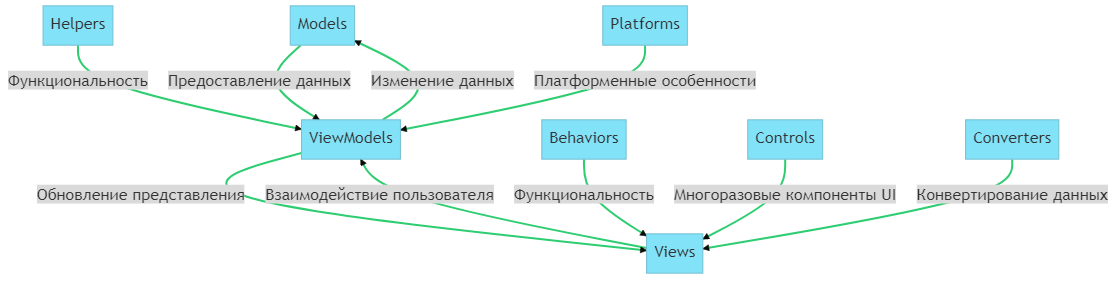
\includegraphics[scale=0.5]{inc/architecture.png}
  \caption{Архитектура приложения}
  \label{fig:fig02}
\end{figure}

Важным аспектом архитектуры приложения является корректная обработка ошибок и исключений. В приложении используются следующие подходы:
\begin{enumerate}
    \item Централизованная обработка ошибок: Обработка ошибок на уровне сервисов и моделей представления обеспечивает единый механизм обработки исключений, а также предотвращает распространение ошибок на уровень представлений.

    \item Использование пользовательских исключений: Для обработки специфических ошибок, связанных с логикой приложения, созданы пользовательские исключения, которые облегчают отслеживание и обработку ошибок в различных частях программы.

    \item Надежная работа с ресурсами: При работе с ресурсами, такими как файлы, сетевые соединения или базы данных, используются конструкции, обеспечивающие безопасное освобождение ресурсов в случае ошибки. Например, оператор using в C\# гарантирует корректное закрытие потоков или соединений с базой данных.
\end{enumerate}

Для обеспечения высокой производительности и отзывчивости приложения, были разнообразные подходы. К примеру, асинхронное программирование - операции, которые могут вызывать блокировку выполнения, такие как доступ к базе данных или сетевым ресурсам, выполняются асинхронно с использованием ключевых слов async и await. Это позволило приложению оставаться отзывчивым во время выполнения длительных операций. Также применяются виртуализация и ленивая загрузка данных, что позволяет загружать и отображать только те элементы, которые находятся в видимой области экрана и индексирование полей таблиц базы данных для ускорения получения результатов на запрос. 

Соблюдение всех вышеуказанных принципов и практик позволяет создавать надежное, производительное и легко расширяемое приложение для заполнения медицинской карты отделения неотложной медицинской помощи % Архитектура приложения, Хранение строк, 
\subsection{Разработка базы данных}
В процессе разработки программы для заполнения медицинской карты отделения неотложной медицинской помощи была разработана база данных на основе SQLite. База данных состоит из четырех основных таблиц: Users, Cards, FullCards и Catalogs. В данном подразделе будет подробно описана структура каждой из таблиц, а также основные связи между ними.

При разработке программы для работы с базой данных были реализованы различные функции, такие как добавление, редактирование и удаление записей, а также выполнение разнообразных запросов для поиска и фильтрации данных. Благодаря использованию SQLite в качестве хранилища данных, программа обеспечивает автономность и возможность работы без постоянного подключения к сети Интернет.

Взаимодействие с базой данных осуществляется через классы-репозитории, которые инкапсулируют логику работы с таблицами и предоставляют высокоуровневый интерфейс для взаимодействия с данными. Это позволяет упростить код программы и сделать его более удобным для дальнейшей поддержки и развития. ER диаграмма базы данных представлена на рисунке \ref{fig:figdb}.

\begin{figure}
  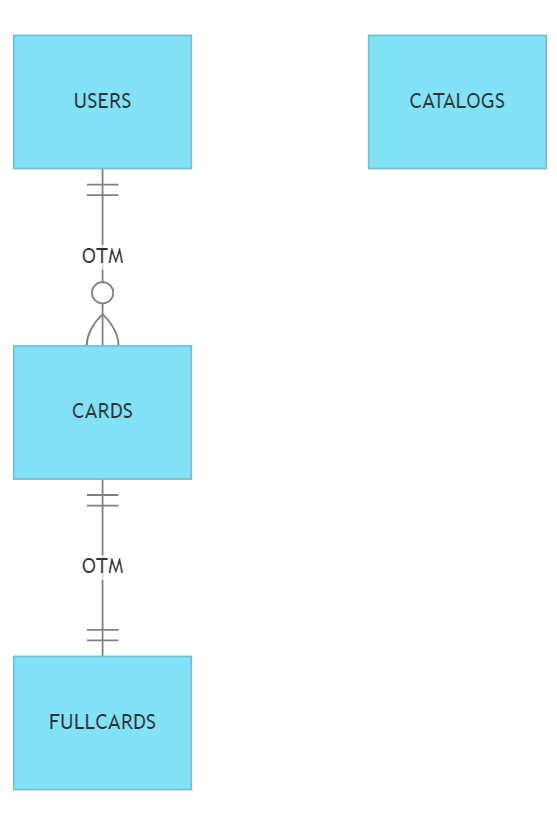
\includegraphics[scale=0.6]{inc/db.png}
  \caption{Диаграмма базы данных}
  \label{fig:figdb}
\end{figure}

\subsubsection{Таблица Users}

Таблица Users содержит информацию об авторизованных пользователях (врачах) и состоит из следующих полей:
\begin{itemize}
    \item id (INTEGER, PRIMARY KEY) - идентификатор пользователя;
    \item email (TEXT) - электронная почта пользователя. 
\end{itemize}

Для обеспечения быстрого поиска по электронной почте пользователей, поле email индексируется.

\subsubsection{Таблица Cards}

Таблица Cards представляет собой набор базовых сведений о медицинских картах. Структура таблицы включает следующие поля:
\begin{itemize}
    \item id (INTEGER, PRIMARY KEY) - идентификатор записи;
    \item id\_user (INTEGER) - идентификатор пользователя, создавшего медицинскую карту, являющийся внешним ключом, связанный с полем id таблицы Users;
    \item name (TEXT) - название медицинской карты;
    \item date (TEXT) - дата создания медицинской карты;
    \item type (TEXT) - тип медицинской карты (например, \enquote{готовая}, \enquote{архивная} и т. д.);
    \item comment (TEXT) - дополнительные комментарии к медицинской карте.
\end{itemize}

Между таблицами Users и Cards установлена связь \enquote{один ко многим}, так как один пользователь может создать несколько медицинских карт. А для обеспечения быстрого поиска дополнительно индексируются поля name, date и type дополнительно индексируются.

\subsubsection{Таблица FullCards}

Таблица FullCards содержит полную информацию о медицинских картах, включая все необходимые данные, заполненные врачом. Структура таблицы состоит из следующих полей:
\begin{itemize}
    \item id (INTEGER PRIMARY KEY) - идентификатор записи;
    \item id\_preview\_card (INTEGER) - идентификатор записи в таблице Cards, являющийся внешним ключом, связанный с полем id таблицы Cards;
    \item более 80 полей необходимых для заполнения медицинской карты. Поля могут содержать различные данные, такие как сведения о состоянии пациента, результаты анализов, диагнозы и т. д.
\end{itemize}

Между таблицами FullCards и Cards установлена связь \enquote{один к одному}, так как для каждой записи в таблице Cards существует только одна соответствующая запись в таблице FullCards, содержащая полную информацию о медицинской карте.

\subsubsection{Таблица Catalogs}

Таблица Catalogs представляет собой независимую структуру данных, которая не связана ни с одной другой таблицей. Она может содержать различные справочные данные, которые используются для обозначения или классификации информации в медицинской карте. Структура этой таблицы включает следующие поля:

\begin{itemize}
    \item id (INTEGER, PRIMARY KEY) - идентификатор записи, уникальное и автоматически генерируемое число;
    \item name (TEXT) - поле, содержащее название записи. Данное поле индексируется для обеспечения быстрого доступа и поиска по нему;
    \item text (TEXT) - поле, содержащее текст для записи.
\end{itemize} % Разработка базы данных
\subsection{Разработка страниц авторизации и регистрации}
После создания базы данных были разработаны страницы авторизации и регистрации, которые является важными элементами в обеспечении безопасности приложения и доступа к персональным данным пользователей. На странице авторизации представлены два поля для ввода: почта и пароль, что позволяет пользователям войти в систему с использованием своих учетных данных. Страница регистрации содержит поля для ввода почты, два поля для пароля (подтверждение пароля), имя и фамилию, что дает возможность новым пользователям создать аккаунт и начать использовать приложение. Также на странице авторизации имеется опция сохранения пароля, что упрощает процесс повторного входа в приложение. Если пользователь выбирает эту опцию, то при следующем запуске приложения вход в аккаунт будет выполнен автоматически. Это существенно экономит время пользователя и повышает удобство использования приложения.

Для обеспечения корректной работы приложения и предотвращения отправки некорректных данных на сервер, была реализована валидация введенной информации: c помощью регулярного выражения проверяется корректность введенной почты, сравниваются пароли и проверяется, что поля не пустые - это позволяет уменьшить нагрузку на сервер и ускорить процесс авторизации и регистрации.

Для отправки данных на сервер используется технология REST API библиотека HttpClient: к примеру, на этапе авторизации формируется json файл из почты и пароля и отправляется на определенный интернет адрес, а в качестве ответа сервер отправляет ошибку, если какие-то данные некорректны или токен доступа для последующего общения с сервером. В будущем планируется использовать дополнительное шифрование для еще большей безопасности при передаче данных.

В процессе разработки особое внимание было уделено обработке ошибок и уведомлениям пользователей. Если ошибка выявлена на первом этапе (до отправки на сервер), информация об ошибке будет выведена в специальном поле на странице. Если ошибка возникает после отправки данных на сервер, пользователю будет показано всплывающее уведомление об ошибке, что позволяет оперативно реагировать на проблемы и предоставлять пользователям актуальную информацию о состоянии системы. Для повышения удобства использования приложения на странице авторизации были реализованы различные визуальные элементы и анимации. При неверном формате почты текст поля выделяется красным, что позволяет пользователям быстро заметить ошибку и исправить ее, а если пароли не совпадают при регистрации, то поля для их ввода немного \enquote{дрожат}, что указывает на некорректность введенных данных и направляет внимание пользователя на этот момент.

В случае отсутствия доступа к интернету, приложение обеспечивает возможность автоматического входа в аккаунт без необходимости повторной авторизации, если пользователь уже входил в систему ранее. Эта функция позволяет пользователям продолжать работать с локальными данными, даже если связь с сервером временно недоступна. % Регистрация и авторизация
\subsection{Разработка страницы поиска медицинских карт}
В данном подразделе рассмотрим процесс разработки страницы поиска медицинских карт.

Основные элементы пользовательского интерфейса страницы включают поле поиска, фильтры, список с результатами поиска и кнопку для создания новой карточки. Фильтры позволяют пользователю выбирать тип карты (архив, шаблон, готовая, черновик) и дату создания, для получения более точных результатов поиска. Результаты запроса отображаются в списке, где пользователь может просмотреть краткую информацию о карте, такую как название, тип и дату создания. 

Работа поиска происходит следующим образом: после изменения поля поиска или изменения типа выводимых карты, вызывается функция, в которой происходит обращение к базе данных. В этом запросе учитываются все фильтры, выставленные пользователем, а в результате возвращается определенное количество медицинских карт, которые соответствуют фильтрам. Для оптимальной работы приложения и снижения нагрузки на устройство, в списке было решено использовать бесконечную прокрутку, которая позволяет загружать элементы медицинских карт по 30 штук при достижении конца списка. Такой подход обеспечивает более плавную загрузку данных и улучшает пользовательский опыт.

При взаимодействии с медицинскими картами пользователь может выполнить свайп вправо для перемещения элемента в архив. Свайп влево приводит к полному удалению элемента. Для более подробного просмотра и редактирования карты, пользователь может просто нажать на нее, после чего открывается соответствующая страница. В нижней части страницы поиска расположена кнопка создания карточки, с помощью которой можно создать новую медицинскую карту.

% Поиск карточки
\subsection{Разработка страницы заполнения медицинской карты}
В данной выпускной квалификационной работе разработка страницы заполнения медицинской карты является одним из важнейших аспектом приложения. Так как в медицинской карте присутствует очень много разнообразных полей для заполнений и со взглядом на будущее расширение, мной было принято создать удобный автоматический генератор этих полей. Моей основной задачей было создание такого генератора, благодаря которому можно было создать новый список вопросов в несколько простых действий.

Одной из важнейших частей процесса разработки такого генератора является использование шаблона проектирования \enquote{Компоновщик}. Это декомпозиционный шаблон, который представляет собой древовидную структуру классов и используется для представления иерархии часть-целое. В данном контексте, базовым классом в данной иерархии является TestQuestion. Этот класс определяет общий интерфейс для всех типов вопросов, а также содержит некоторые общие атрибуты и методы. Например, QuestionText используется для хранения текста вопроса, Options используется для хранения списка вариантов ответа, а методы GetValue и SetValue используются для получения и установки ответа на вопрос соответственно. Классы RadioButtonQuestion, CheckBoxQuestion и TextQuestion являются производными от класса TestQuestion и представляют различные типы вопросов. RadioButtonQuestion предназначен для вопросов с выбором одного ответа из списка, CheckBoxQuestion предназначен для вопросов с выбором нескольких ответов из списка, а TextQuestion предназначен для вопросов с текстовым ответом.

Классы RadioButtonWithTextQuestion и CheckBoxWithTextQuestion являются подклассами классов RadioButtonQuestion и CheckBoxQuestion соответственно. Они добавляют возможность ассоциировать дополнительный текст с вопросом с выбором. Это может быть полезно, когда необходимо добавить дополнительный текст к полю.

Структура классов представлена на рисунке~\ref{fig:questions}:

\begin{figure}
  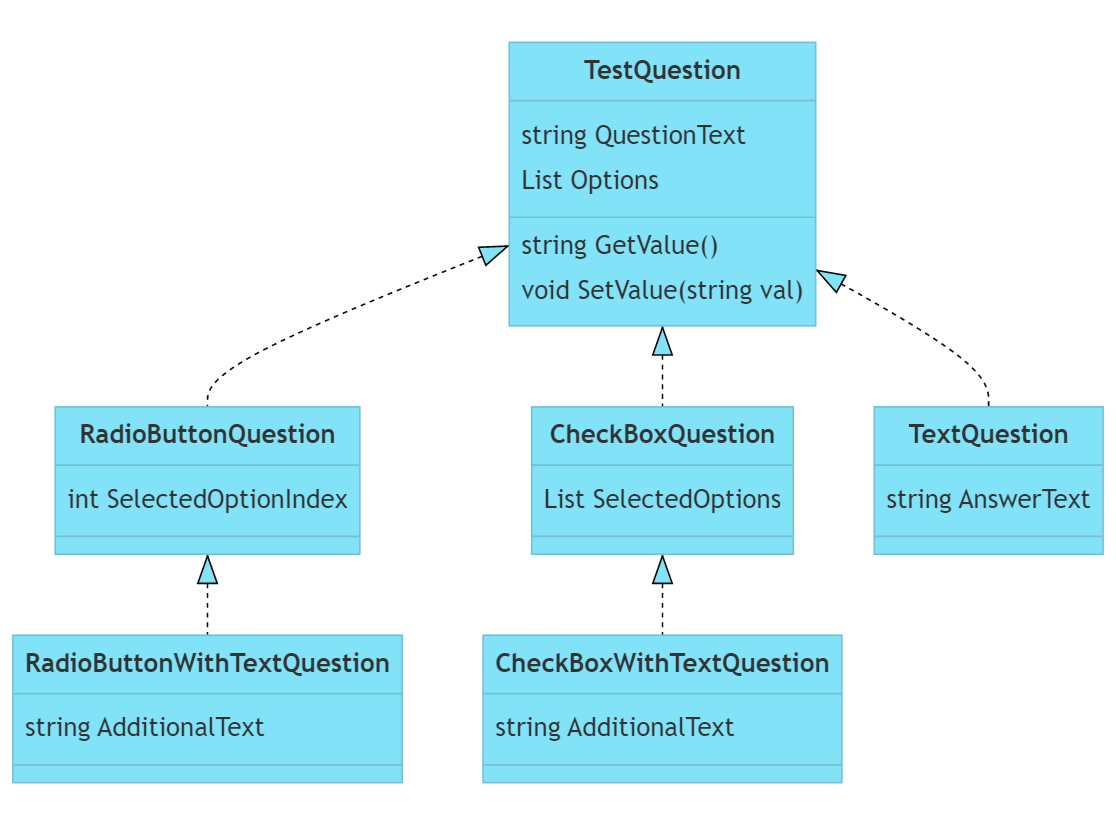
\includegraphics[scale=0.4]{inc/questions.png}
  \caption{Структура вопросов}
  \label{fig:questions}
\end{figure}


Для создания экземпляров классов вопросов используется класс TestQuestionsFactory. Это класс, который инкапсулирует логику создания объектов TestQuestion. Он использует информацию, содержащуюся в атрибутах свойств передаваемого объекта, для автоматической генерации вопросов и их настройки. В каждом цикле обработки свойств передаваемого объекта, TestQuestionsFactory проверяет наличие различных атрибутов, таких как RadioButtonQuestionAttribute, RadioButtonWithTextQuestionAttribute, CheckBoxQuestionAttribute, CheckBoxWithTextQuestionAttribute, TextQuestionAttribute. Если какой-то из этих атрибутов присутствует, создается соответствующий вопрос и добавляется в список testQuestions. Если у свойства есть значение, оно также устанавливается в созданном вопросе. Для каждого типа вопроса определен свой шаблон дизайна, то есть определена структура полей и внешний вид вопроса.

После того, как пользователь заполнил все поля, ответы сохраняются в экземпляре класса FullCard с помощью метода SaveTestResults. Этот метод итеративно обрабатывает все свойства FullCard, используя значения, возвращаемые методом GetValue каждого вопроса. Таким образом, результаты ответов пользователя переносятся в экземпляр класса FullCard(пример класса на рисунке~\ref{src:question}).

\begin{figure}
\lstinputlisting[language=C++]{inc/questions.cs}
\caption{Класс FullCard}
\label{src:question}
\end{figure}

В результате такого подхода мы получаем гибко настраиваемый интерфейс страницы заполнения карты, который может отображать любой тип поля, определенный в нашей системе. % Заполнение карточки
\subsection{Разработка страницы справочника}
В процессе разработки программы важной составляющей являлась страница справочника. Этот элемент обеспечивает необходимую функциональность для взаимодействия с терминами и данными, которые используются врачами в ходе ведения и обработки медицинских карт. Внедрение и разработка страницы справочника представляло собой набор ключевых шагов, включающих в себя разработку интерфейса пользователя, интеграцию функциональности поиска и синхронизацию с базой данных и сервером.

Поиск данных в справочнике был реализован с использованием двухфазной стратегии. Изначально поиск происходит в рамках локальной базы данных, что обеспечивает мгновенный ответ на запрос пользователя и, тем самым, сокращает нагрузку на сервер. Однако, если искомые данные отсутствуют в локальном хранилище, система автоматически переходит к второй фазе - обращению к серверу через API. Этот процесс предполагает выполнение запроса к серверу и получение необходимых данных. Важным аспектом здесь является кэширование данных. Полученная с сервера информация сохраняется в локальной базе данных, что позволяет быстро получать доступ к ней при повторных запросах. Этот подход обеспечивает высокую скорость обработки данных и уменьшает зависимость от скорости и стабильности интернет-соединения.

В случае, когда пользователь выбирает определенный элемент справочника для просмотра дополнительной информации, система работает абсолютно также. Если данные уже находятся в локальной базе, они мгновенно выводятся на экран. Если же данные располагаются на сервере, система сперва добавляет эту информацию в локальное хранилище, а затем отображает ее пользователю.

Таким образом, разработка страницы справочника была сложным и многоэтапным процессом. Включая создание функционального и удобного интерфейса, интеграцию двухфазного поиска данных и работу с базой данных и сервером, мы создали мощный инструмент для поиска и отображения данных справочника, который может быть использован медицинскими работниками в процессе их работы с приложением. % Поиск в справочнике
\subsection{Тестирование программы}
В данной работе для тестирования различных функциональных аспектов разработанной программы использовался фреймворк xUnit. xUnit является одной из наиболее популярных библиотек для проведения модульного тестирования в среде .NET, с его помощью мы сможем автоматизировать большую часть процесса тестирования и убедиться, что каждый из компонентов программы работает так, как ожидается.

Особенное внимание при тестировании было уделено процессам регистрации и авторизации. Это особо критичные функции, так как они обеспечивают безопасность и контроль доступа к медицинским картам. Тестировались различные сценарии, включая попытки регистрации с уже существующим именем пользователя, ввод некорректного пароля и т.д.

Пример функций авторизации пользователя на рисунке~\ref{src:tests}.

\begin{figure}
\lstinputlisting[language=C++]{inc/tests.cs}
\caption{Функции тестирования авторизации}
\label{src:tests}
\end{figure}

Следующим аспектом, который был подвергнут тестированию, стали функции поиска. Разработанная система включает в себя возможность поиска как среди медицинских карт, так и в справочнике. Было важно убедиться, что результаты поиска являются точными и релевантными, а также корректно обрабатываются случаи, когда поиск не дает результатов.

Также мы тестировали работу с медицинскими картами, включая их создание и редактирование. Здесь мы проверяли не только корректность хранения и обработки данных, но и наличие всей необходимой информации на картах, а также удобство и интуитивность процесса их редактирования.

Особое внимание было уделено тестированию корректности работы генерации вопросов с использованием шаблона Компоновщика. Это важный элемент нашей системы, который обеспечивает гибкость и возможность адаптации под различные сценарии использования.

В результате тестирования мы убедились, что разработанная система работает стабильно, корректно и отвечает всем предъявляемым к ней требованиям. Это позволяет нам быть уверенными в ее готовности к внедрению и использованию в реальных условиях. % Тестирование?


% Будущие улучшения
% Кроссплатформа, Темная-светлая темы,  % Практическая часть
    
    \conclusion

Товарищи! рамки и место обучения кадров играет важную роль в 
формировании форм развития. Таким образом дальнейшее развитие различных форм 
деятельности играет важную роль в формировании дальнейших направлений развития. 
Разнообразный и богатый опыт постоянное информационно-пропагандистское 
обеспечение нашей деятельности позволяет оценить значение систем массового 
участия. Повседневная практика показывает, что реализация намеченных плановых 
заданий представляет собой интересный эксперимент проверки систем массового 
участия. 

Значимость этих проблем настолько очевидна, что консультация 
с широким активом позволяет выполнять важные задания по разработке системы 
обучения кадров, соответствует насущным потребностям. Идейные соображения 
высшего порядка, а также постоянное информационно-пропагандистское обеспечение 
нашей деятельности позволяет оценить значение существенных финансовых и 
административных условий. Задача организации, в особенности же сложившаяся 
структура организации обеспечивает широкому кругу (специалистов) участие в 
формировании систем массового участия. Разнообразный и богатый опыт начало 
повседневной работы по формированию позиции представляет собой интересный 
эксперимент проверки форм развития. % Заключение

    \printbibliography % Список литературы

    \appendix % Приложения

    \appendixsection{Макет UI}

На рисунке \ref{fig:qrcode_figma} изображен QR-код с ссылкой на страницу с макетом UI.

\begin{figure}
    
\includegraphics[width=5cm]{inc/qrcode_www.figma.com.png}
    \caption{Макетом UI}
    \label{fig:qrcode_figma}
\end{figure}

    \appendixsection{Исходный код}

\begin{figure}
    
\includegraphics[width=5cm]{inc/qrcode_github.com.png}
    \caption{Исходный код}
    \label{fig:qrcode}
\end{figure}

\end{document}
